The language of \textsc{EviL} is evidently modal, and in previous
sections the semantics have largely suggested that there are clear
connections to conventional Kripke semantics.  
In this section, we will demonstrate that every \textsc{EviL} model
corresponds to some highly structured Kripke model, with a minor
modification on the standard definition.  However, it will turn out
that this correspondence is one way - the class of Kripke models for
which \textsc{EviL} is strongly complete do not, in general,
possess corresponding \textsc{EviL} models.

In order to understand \textsc{EviL} models as
Kripke models, we return to the visualization technique for
\textsc{EviL} models we introduced in \S\ref{quine}.  There
we suggested that \textsc{EviL} models can be thought of as 
\emph{posets}, with the partial ordering corresponding to set
containment.  Here we make the added requirement that the worlds
remain in this ordering.  In addition, doxastic accessibility will be
visualized with arrows. We can see examples of this visualization
technique below in 
Figs. \ref{fig:example2}  and \ref{fig:example3}.  

In the interest of being completely explicit, these
figures should be read as follows:
\begin{bul}
 \item if one point $(a,A)$ is above another point $(b,B)$ and
   connected by a densely dotted line 
   \tikz \draw[densely dotted,semithick](0pt,0pt) -- (20pt,6pt);, 
   this means that $a = b$ and $B \subset A$.
  \item if one point $(a,A)$ is connected to another point $(b,B)$ by
    a line with an arrow \tikz \draw[->,>=latex,semithick](0pt,0pt) --
    (20pt,6pt);, this means that $\Omega,(b,B) \VDash A$
\end{bul}
In all of these depictions, the implicit relational structure of 
\textsc{EviL} models is given visual expression.  So it seems 
only natural that this graphically perceived structure
could also find formal expression.

\begin{figure}[ht]
\centering
\subfigure[A fairly simple example]{
  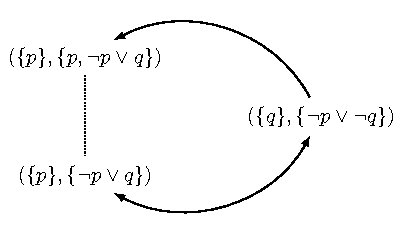
\includegraphics[]{evil_pictures/first_fig.pdf}
\label{fig:example2}
}
\subfigure[A more complex example]{
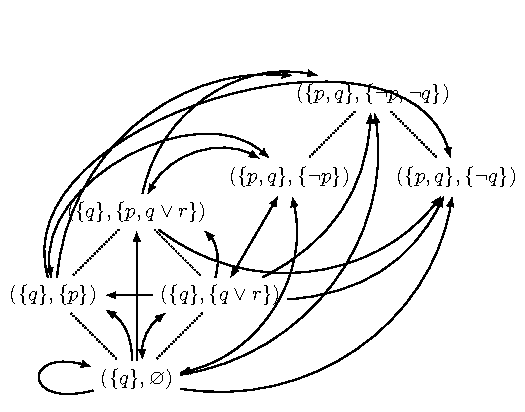
\includegraphics[]{evil_pictures/second_fig.pdf}
\label{fig:example3}
}
\caption{\textsc{EviL} model visualizations}
\end{figure}

Following the modified semantics provided in \S\ref{multi-agent}, the
developments this section will assume multiple agents.
\begin{definition}
  Let $\Phi$ be a set of letters and let $\mathcal{A}$ be a set of agents. 
  A \textbf{Kripke structure} is a state transition system
  $\mathbb{M}=\langle W^\mathbb{M}, R^\mathbb{M},
  \sqsubseteq^\mathbb{M}, \sqsupseteq^\mathbb{M}, V^\mathbb{M},
  P \rangle$ where\footnote{Where
    the context is clear, we shall drop the superscript $\mathbb{M}$.}:
  \begin{itemizedot}
    \item $W$ is a set of worlds    
    \item $R : \mathcal{A} \rightarrow \powerset (W \times W)$, $\sqsubseteq : \mathcal{A} \rightarrow \powerset (W \times W)$, and $\sqsupseteq : \mathcal{A} \rightarrow \powerset (W \times W)$ are
    $\mathcal{A}$-indexed sets of relations\footnote{We shall abbreviate
      $R(X)$, $\sqsubseteq(X)$, $\sqsupseteq(X)$, $P(X)$ as $R_X$,
      $\sqsubseteq_X$, $\sqsupseteq_X$ and $P_X$ respectively}
    \item $V : \Phi \rightarrow \powerset (W)$ is a predicate letter valuation
    \item $P : \mathcal{A} \rightarrow \powerset
      (W)$ are sets of worlds indexed by agents
  \end{itemizedot}
  Let $\mathcal{K}_{\Phi, \mathcal{A}, I}$ denote the class of Kripke structures for letters $\Phi$, agents $\mathcal{A}$, and where $W \subseteq I$.
\end{definition}
% \begin{definition}
% By a minor abuse of notation, 
% we shall write $w \sqsubseteq v$ to mean that $w
% \sqsubseteq_X v$ for all agents $X$.
% \end{definition}

The Kripke semantics given by $(\Vdash) \colons \mathcal{K}_{\Phi, \mathcal{A}, I} \to I
\rightarrow \mathcal{L}(\Phi, \mathcal{A}) \to \text{\tmtextsf{bool}}$ for these models are defined recursively
as usual, granting the exceptional behavior of $P$.
\begin{definition}
  Let $\mathbbm{M}$ be a Kripke structure:
  \begin{eqnarray*}
    \mathbbm{M}, w \Vdash p & \Longleftrightarrow & w \in V
    (p)\\
    \mathbbm{M}, w \Vdash \phi \rightarrow \psi & \Longleftrightarrow &
    \mathbbm{M}, w \Vdash \phi \text{ implies } \mathbbm{M}, w \Vdash \psi\\
    \mathbbm{M}, w \Vdash \bot & \Longleftrightarrow & \text{False}\\
    \mathbbm{M}, w \Vdash \Box_X \phi & \Longleftrightarrow & \forall v \in
    W . w R_X v \text{ implies } \mathbbm{M}, v
    \Vdash \phi\\
    \mathbbm{M}, w \Vdash \boxminus_X \phi & \Longleftrightarrow & \forall v
    \in W . w \sqsupseteq_X v \text{ implies }
    \mathbbm{M}, v \Vdash \phi\\
    \mathbbm{M}, w \Vdash \boxplus_X \phi & \Longleftrightarrow & \forall v
    \in W . w \sqsubseteq_X v \text{ implies }
    \mathbbm{M}, v \Vdash \phi\\
    \mathbbm{M}, w \Vdash \circlearrowleft_X & \Longleftrightarrow & w \in
    P_X
  \end{eqnarray*}
\end{definition}
Kripke structures can be observed to typically have a lot less structure than
\tmtextsc{EviL} models.  On the other hand,  \tmtextsc{EviL} models
can be understood as Kripke structures in disguise.  To illustrate
this, observe the following lemma:
\begin{definition}[$\mho^\Omega$ Translation]\label{omega-translation}
Let $\Omega$ be an \tmtextsc{EviL} model.  Define
  $\mho^{\Omega} \assign \langle \Omega, R^{\Omega},
  \sqsubseteq^{\Omega}, \sqsupseteq^{\Omega}, V^{\Omega},
  P^{\Omega} \rangle$, where
  \[ \begin{array}{llll}
       \bullet & \text{$(a, A) R^{\Omega}_X (b, B) \Longleftrightarrow \forall
       \psi \in A_X .b \models \psi$} & \bullet & (a, A)
       \sqsubseteq^{\Omega}_X (b, B) \Longleftrightarrow a = b \text{ and }
       A_X \subseteq B_X\\
       \bullet & (a, A) \sqsupseteq^{\Omega}_X (b, B) \Longleftrightarrow a =
       b \text{ and } A_X \supseteq B_X & \bullet & (a, A) \in
       P^{\Omega} (X) \Longleftrightarrow \forall \psi \in
       A_X .a \models \psi \\
\multicolumn{4}{c}{\bullet\ \ \ V(p) := \{ (a,A) \in \mathfrak{M} \ |\ \mathfrak{M},(a,A)\VDash p\}}
     \end{array} \]
\end{definition}
\begin{lemma}
  \label{tranlemma1} For all $\Omega$ and all $(a, A) \in \Omega$,  
\begin{center} 
$\Omega, (a, A) \VDash \phi$ if and only if $\mho^{\Omega}, (a, A) \Vdash \phi$.
\end{center}
\end{lemma}
\begin{proof}
  This follows from a straightforward induction on $\phi$.
\end{proof}
The following summarizes the structural properties of
\tmtextsc{EviL} models, when transformed into Kripke structures:
\begin{proposition}\label{evil_models}
  For any \textsc{EviL} model $\Omega$,  $\mho^{\Omega}$ has the following
  properties, for all agents $\{X,Y\} \subseteq \mathcal{A}$:
% {\footnote{Note that in this we have that $\{w,v\} \subseteq \powerset
%     \Phi \times \powerset \mathcal{L}_0$ in the subsequent discussion}}
:
  \begin{myRoman}
    \item\label{pI} $\sqsubseteq^{\Omega}_X$ is reflexive
    \item\label{pII} $\sqsubseteq^{\Omega}_X$ is transitive 
%   \item \label{pantisym} $\sqsubseteq^{\Omega}$ is a partial order
    \item \label{preverse} $w \sqsubseteq^{\Omega}_X v$ if and only if 
     $v \sqsupseteq^{\Omega}_X w$
    \item \label{pislandiff} If $w \sqsubseteq^{\Omega}_X v$ then ($w
      \in V (p)$ if and only if $v \in V (p)$)
    \item \label{pV}$(R^{\Omega}_X \circ \sqsubseteq^{\Omega}_X) \subseteq R^{\Omega}_X$
    \item \label{pVI} $(\sqsubseteq^{\Omega}_Y \circ R^{\Omega}_X)
      \subseteq R^{\Omega}_X$ and\\
    $(\sqsupseteq^{\Omega}_Y \circ R^{\Omega}_X) \subseteq
    R^{\Omega}_X$
    \item\label{pVII} $w \in P^{\Omega} (X)$ if and only if $w
    R^{\Omega}_X w$
  \end{myRoman}
  The situation in \ref{pV} can be visualized in a commutative diagram
  depicted in
  \ref{fig:commut1}, while \ref{pVI} can be split into
  Figs. \ref{fig:commut2} and \ref{fig:commut3}.
\end{proposition}
\begin{figure}[ht]
\centering
\subfigure[\ --\ \ref{pV}\ --\ \newline 
$(R^{\Omega}_X \circ \sqsubseteq^{\Omega}_X) \subseteq
R^{\Omega}_X$]{
  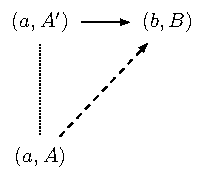
\includegraphics[]{commutative/commutative1.pdf}
%\caption{A fairly simple example}
\label{fig:commut1}
}
\hspace{1cm}
\subfigure[\ --\ \ref{pVI}\ --\ \newline 
 $(\sqsubseteq^{\Omega}_Y \circ R^{\Omega}_X) \subseteq
 R^{\Omega}_X$ 
]{
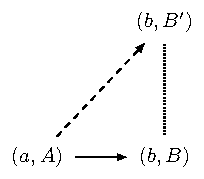
\includegraphics[]{commutative/commutative2.pdf}
\label{fig:commut2}
}
\hspace{1cm}
\subfigure[\ --\ \ref{pVI}\ --\ \newline  
$(\sqsupseteq^{\Omega}_Y \circ R^{\Omega}_X) \subseteq
R^{\Omega}_X $]{
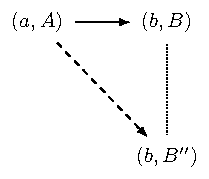
\includegraphics[]{commutative/commutative3.pdf}
\label{fig:commut3}
}
\caption{Visualizations of the relationships in Proposition \ref{evil_models}}
\end{figure}
\begin{proof}
  Everything except \ref{pV} and \ref{pVI} follows directly
  immediately from the definitions:
\begin{description}
  \item[\ref{pV}] We must show
$(R^{\Omega}_X \circ \sqsubseteq^{\Omega}_X) \subseteq R^{\Omega}_X$.
  
  Assume that $(a, A) \sqsubseteq_X^{\Omega} (b, B) R_X^{\Omega} (c,C) $, then evidently $\forall \psi \in
  B_X .c \models \psi$. Since $A_X \subseteq B_X$ then evidently $\forall \psi \in
  A_X .c \models \psi$.  This means that $(a,A) R^{\Omega}_X (c,C)$,
  which suffices the claim.
  
\item[\ref{pVI}] We must show:
\begin{eqnarray*}
 & (\sqsubseteq^{\Omega}_Y \circ R^{\Omega}_X)
       \subseteq R^{\Omega}_X\\
& \& \\
&  (\sqsupseteq^{\Omega}_Y \circ R^{\Omega}_X) \subseteq R^{\Omega}_X 
\end{eqnarray*}

So assume either of the following:
\begin{eqnarray*}
&(a,A) R^{\Omega}_X (b,B) \sqsubseteq^{\Omega}_X (c,C)\\
&\textup{or} \\
&(a,A) R^{\Omega}_X (b,B) \sqsupseteq^{\Omega}_X (c,C)
\end{eqnarray*}

In either case we have that $\forall \psi \in
  A_X .b \models \psi$, and moreover $b =c$.  Hence $\forall \psi \in
  A_X .c \models \psi$, which means that $(a,A) R^{\Omega}_X (c,C)$,
  which was what was to be shown.
\end{description}
\end{proof}

\begin{definition}\label{evil-kripke-structures}
A Kripke structure is called \textsc{EviL} if it makes true the
  above properties \ref{pI} through \ref{pVII}.
\end{definition}

% These properties are definitive - as shall be demonstrated in \S\ref{Abstract-Completeness}, \tmtextsc{EviL} is
% sound and strongly complete for \tmtextsc{EviL} models.

The Kripke semantics provide proper intuition behind
\tmtextsc{EviL} models. We think of the defined relations given as follows:
\begin{itemizedot}
  \item If $x R^{\Omega}_X y$, then at world $x$ the agent $X$ can imagine $y$ is true, since $y$ is compatible with what the agent believes 
  \item If $x \sqsubseteq^{\Omega}_X y$, then agent $X$'s
  assumptions at world $x$ (or the experiences they are taking under consideration) are  contained in her evidence at $y$
\end{itemizedot}
Given this perspective, the proof of \ref{pV} can be understood in the
following way - if the agent assumes fewer things, more things are imaginable,
since it is easier for a world to be incompatible with an agent's evidence.

Finally, while Prop. \ref{evil_models} presents itself as a sort of
representation lemma, the relationship between \textsc{EviL} semantics
and Kripke semantics is not reciprocal.  Proposition
\ref{not-an-evil-model} shows that not every Kripke model can be
represented as an \textsc{EviL} model, 
by presenting an elementary example of  this failure of
representation.  It turns on the following observation:

\begin{lemma}\label{helper-lemma}
  For a given \textsc{EviL} model $\mathfrak{M}$, for any
  $\{(a,A),(b,B),(c,C)\} \subseteq \mathfrak{M}$, if $a = b$ then $a
  \models C$ if and only if $b \models C$.
\end{lemma}
\begin{proof}
  Recall that the semantics for $\models$, as defined in Definition
  \ref{classical-semantics} in \S\ref{evil-grammar} are the usual
  semantics for classical propositional logic. Remembering this, the
  above is an elementary result in basic logic.
\end{proof}

\begin{proposition}[Failure of Representation]
\label{not-an-evil-model}
 Not every \textsc{EviL} Kripke structure has a representative \textsc{EviL} model.
\end{proposition}
%\end{lemma}
%\begin{proof}
\begin{proof}
Consider a single agent \textsc{EviL} Kripke structure $\mathbb{M}:=\langle W, R,
  \sqsubseteq, \sqsupseteq, V, P \rangle$ where
\begin{center}
\begin{tabular}{ l c l }
 \quad $W := \{w,v\}$ & & $\sqsubseteq := \sqsupseteq := \{(w,w),(v,v)\}$ \\
 \quad $R := \{(w,v)\}$ & & $V(p) := \varnothing$ for all $p\in \Phi$ \\
   & $P := \varnothing$ & \\
\end{tabular}
\end{center}
This structure is depicted in Fig. \ref{fig:notevil}.  We shall show
that $\mathbb{M}$ is not represented 
by any \textsc{EviL} model.

Observe that $\mathbb{M}$ makes true the following:
\begin{align}
  \mathbb{M},w & \Vdash \Pos \top \label{notevil:eq1}\\
  \mathbb{M},w & \Vdash \Nec \neg p \textup{ for all $p \in
    \Phi$} \label{notevil:eq4} \\
  \mathbb{M},w & \Vdash \neg p \textup{ for all $p \in \Phi$} \label{notevil:eq2} \\
  \mathbb{M},w & \Vdash \neg \Pos \Pos \top \label{notevil:eq3} 
\end{align}
Armed with these observations, we can assert that it is impossible for
there to be an \textsc{EviL} structure $\mathfrak{M}$ with a world
$(a,A)$ such that $\mathbb{M},w \Vdash \phi$ if and only if
$\mathfrak{M}, (a,A) \VDash \phi$.

For suppose there were, then we could deduce the following facts, using
the observations above:
\begin{mynum}
\item\label{notevil:1} From \eqref{notevil:eq1}, there must be some pair $(b,B)
   \in \mathfrak{M}$ such that $b\models A$.  Hence, $A$ must be
   \emph{consistent}.
\item From \eqref{notevil:eq4}, we know that for the $b$ mentioned above it must be that $b = \varnothing$. This is a
  direct consequence of Lemma \ref{truthiness}, the Truthiness Lemma.
 \item From \eqref{notevil:eq2}, evidently $a = \varnothing$
  \item From \eqref{notevil:eq3}, it must be
    that $a \nmodels A$. Otherwise by the semantics of
    \textsc{EviL} as defined in \S\ref{evil-grammar} we would have
    $\mathfrak{M},(a,A) \VDash \Pos \Pos \top$
\end{mynum}
Since $a = b = \varnothing$ and $b \models A$
then by Lemma \ref{helper-lemma} it must be that $a \models A$. But this
clearly is absurd! $\lightning$
%\end{proof}
\end{proof}

\begin{figure}[ht]
\centering
  
\includegraphics[]{evil_pictures/third_fig.pdf}
%\caption{A fairly simple example}
\caption{A Kripke structure $\mathbb{M}$ with no \textsc{EviL} representation}
\label{fig:notevil}
\end{figure}

The above one way correspondence is admittedly inconvenient - 
it means that while \textsc{EviL} only enjoys some features from
traditional epistemic logic, it is denied others.  Despite this,
\textsc{EviL} enjoys \emph{most} of the benefits of basic modal logic.
Indeed, we shall see in \S\ref{Abstract-Completeness} that
\textsc{EviL} is strongly complete for \textsc{EviL} Kripke models.  

Perhaps the most important formal feature that 
\textsc{EviL} semantics lacks in comparison to 
abstract Kripke semantics is that, as a consequence of the
observations made in
Proposition \ref{not-an-evil-model}, \textsc{EviL} is not compact.

\begin{theorem}[Failure of Compactness]\label{noncompact}If the set of proposition
  letters $\Phi$ is infinite, then
\textsc{EviL} is not compact for \textsc{EviL} semantics.
\end{theorem}
\begin{proof}
We shall prove this result for the single agent case (the multiple
agent case is an obvious generalization).  
Consider the function $\tau : \Phi \to \mathcal{L}(\Phi)$, defined as
follows:
\[ \tau(p) := (\Pos \top) \wedge (\Nec \neg p) \wedge (\neg p) \wedge
(\neg \Pos \Pos \top) \]
We shall see that $\tau[\Phi]$ is finitely satisfiable, but not
in its entirety.

Clearly not all of $\tau[\Phi]$ is satisfiable in \textsc{EviL}
semantics, by the arguments presented in the proof of Proposition \ref{not-an-evil-model}.

Now consider some finite subset of $S  \subseteq_\omega \tau[\Phi]$.
We shall construct a model that makes $S$ true. 
Since $\tau$ is injective, we know there is 
some $\Psi \subseteq \Phi$ such that $S = \tau[\Psi]$.  
Since $\Phi$ is infinite, we know there is some $\rho \in \Phi \bs \Psi$.  
Now consider a model $\mathfrak{M} = \{(\{\rho\}, \{\neg \rho\}),
(\varnothing, \{\bot\})\}$.  This is depicted in
Fig. \ref{fig:failureofcompactness}.  It is straightforward to verify
that $\mathfrak{M},(\{\rho\}, \{\neg
  \rho\}) \VDash \tau[\Psi]$, so $\mathfrak{M}$ is a suitable witness.
\end{proof}

\begin{figure}[ht]
\centering
  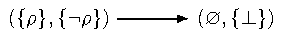
\includegraphics[]{evil_pictures/forth_fig.pdf}
%\caption{A fairly simple example}
\caption{A model $\mathfrak{M}$ where $\mathfrak{M}, (\{\rho\}, \{\neg
  \rho\}) \VDash \tau[\Psi]$ for $\Psi \subseteq_\omega \Phi$ and $\rho \nin \Psi$}
\label{fig:failureofcompactness}
\end{figure}

A consequence of the failure of compactness, while strong
completeness can be obtained for \textsc{EviL} using Kripke semantics,
to achieve completeness for \textsc{EviL} semantics a finitary proof
must be carried out.  Recall that this was exactly the strategy used
in our original sketch of \textsc{EviL} that we gave in Proposition
\ref{translation-sketch} in \S\ref{sketch}.

The next section is devoted to studying completeness for \textsc{EviL}.

% Furthermore, even though \textsc{EviL}
% is quite formal in nature, it might rightly be considered an
% application  of traditional modal logic rather than a novel logic
% in of itself.   The novelty of \textsc{EviL} is that it presents semantics
% that automatically connect truth and derivability (as expressed in
% Theorem \ref{theorem-theorem}, the Theorem Theorem).

%%% Local Variables: 
%%% mode: latex
%%% TeX-master: "evil_philosophy"
%%% End: 
